\section{Finding 10 - Privilige Escalation via SSH}

%center under chapter title a one row table with 6 coloumns and no borders
\vspace*{-0,3cm}
\begin{center}
    \begin{tabular}{c c c c}
        \textbf{Classification:} & Misconfiguration & \textbf{Severity:} & \textbf{\textcolor{red}{High}}  
        \end{tabular}
\end{center}

Within the roots authorized\_keys file in the ”.ssh” directory a public key for the user ”bluey” is stored.
\subsection{Finding Impact}
Doing a simple ssh login the ”bluey” user can login as root without a password. 

\subsection{Finding Details}
The following snippet shows the content of the authorized\_keys file for the root user:
%code snippet
\begin{lstlisting}[language=bash]
$ cat authorized_keys
ssh-ed25519 AAAAC3NzaC11ZDIINTE5AAAAIMOEhQP4e3BVrq0R9nPQzf
olf9349W/UDXSAbQIj6RDM joe@reliant 
ssh-ed25519 AAAAC3NzaC11ZDI1NTE5AAAAINV2RROAIF7+9Cm7U2PWV
TmJOhjvTQeYF04Lo7Et1qk bluey@plunder
\end{lstlisting}

The following screenshot shows the root login as the ”bluey” user:
\begin{figure}[h]
    \centering
    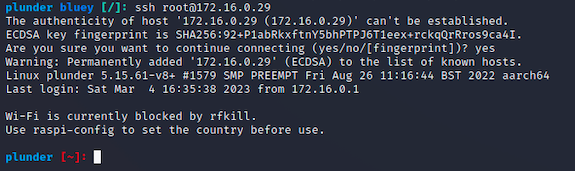
\includegraphics[width=0.8\textwidth]{img/ssh-root-bluey.png}
    \caption{Screenshot of the portscan}
    \label{fig:fin10}
\end{figure}

\subsection{Evaluation of Results}
\begin{center}
    \begin{tabular}{cccc}
    \textbf{Effort to Fix:} & &\ \textbf{\textcolor{blue!50!green}{Low}}\
    \end{tabular}
\end{center}
Remove the public key for the user ”bluey” from the authorized\_keys file for the root user.
